% TEX compiler = latexmk
% copyright arturo salinas-aguayo 2024
\documentclass[12pt]{article}

\usepackage{graphicx}
\usepackage{amsmath}
\usepackage{array}
\usepackage{amsfonts}
\usepackage{fancyhdr}
\usepackage{geometry}
\usepackage{circuitikz}
\usepackage{subfigure}
\usepackage{caption}
\usepackage{karnaugh-map}
\usepackage{bm}
\usepackage[table]{xcolor}
\usepackage{float}
\usepackage{subcaption}

\geometry{letterpaper, margin=1in}
\graphicspath{ {../images/} }

% Header and Footer
\pagestyle{fancy}
\fancyhf{}
\fancyhead[L]{CSE 2301 - Exam 3 Review}
\fancyhead[R]{\thepage}
\setlength{\headheight}{15pt}

\author{Arturo Salinas-Aguayo}
\title{Exam 3 Review}
% theorem set
\newtheorem{example}{Example}
% Example block environment
\newenvironment{examp}
{
	\vspace{.5cm}
	\hrule
\begin{example}\upshape}
	{\hrule
		\vspace{0.5cm}
\end{example}}

\begin{document}
\newcommand{\closure}[2][3]{%
	{}\mkern#1mu\overline{\mkern-#1mu#2}}
\newcommand\ncoverline[1]{\mkern1mu\overline{\mkern-1mu#1\mkern-1mu}\mkern1mu}
% Title Page
\begin{titlepage}
	\centering
	\vspace*{3cm}
	\huge\textbf{Exam 3 Review}\\
	\vspace{5cm}
	\Large\textbf{Arturo Salinas-Aguayo}\\
	\normalsize
	CSE 2301: Principles and Practice of Digital Logic Design\\
	Dr. Mohammad Khan, Section 003L-1248\\
	Electrical and Computer Engineering Department
	\vfill
	\includegraphics[scale=0.1]{uconnlogo}\\
	College of Engineering, University of Connecticut\\
	\scriptsize{Coded in \LaTeX}
	\vspace*{1cm}
\end{titlepage}
\section*{Flip Flop Question}
The operation of the S-R Latch is as follows:

\begin{figure}[H]
	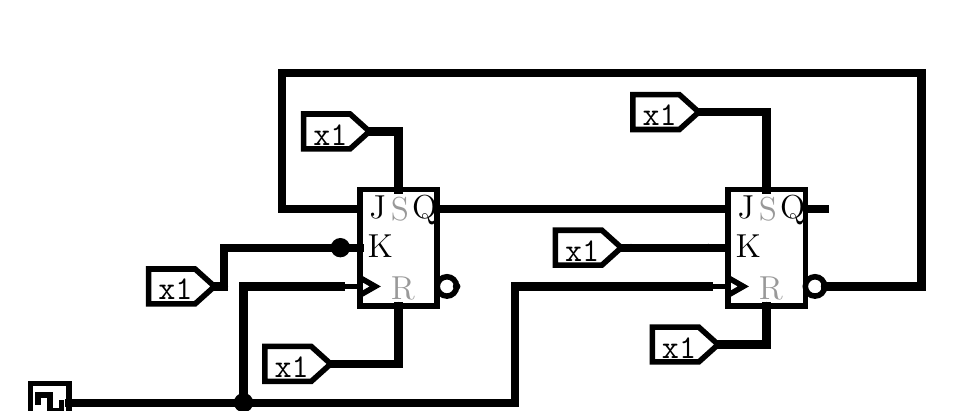
\begin{tikzpicture}[x=1pt,y=-1pt,scale=.7,line cap=rect]
		\def\logisimfontA#1{\fontfamily{cmr}{#1}} % Replaced by logisim, original font was "SansSerif"
		\def\logisimfontB#1{\fontfamily{cmtt}{#1}} % Replaced by logisim, original font was "Monospaced"
		\definecolor{custcol_0_0_0}{RGB}{0, 0, 0}
		\definecolor{custcol_ff_ff_ff}{RGB}{255, 255, 255}
		\definecolor{custcol_99_99_99}{RGB}{153, 153, 153}
		\draw [line width=3.0pt, custcol_0_0_0 ]  (25.0,175.0) -- (115.0,175.0) -- (255.0,175.0) -- (255.0,115.0) -- (355.0,115.0) ;
		\draw [line width=3.0pt, custcol_0_0_0 ]  (165.0,115.0) -- (115.0,115.0) -- (115.0,175.0) ;
		\fill [line width=3.0pt, custcol_0_0_0]  (165.0,95.0) ellipse (5.0 and 5.0 );
		\fill [line width=3.0pt, custcol_0_0_0]  (115.0,175.0) ellipse (5.0 and 5.0 );
		\draw [line width=2.0pt, custcol_0_0_0 ]  (175.0,65.0) -- (214.0,65.0) ;
		\draw [line width=2.0pt, custcol_0_0_0 ]  (215.0,65.0) -- (215.0,124.0) ;
		\draw [line width=2.0pt, custcol_0_0_0 ]  (215.0,125.0) -- (176.0,125.0) ;
		\draw [line width=2.0pt, custcol_0_0_0 ]  (175.0,125.0) -- (175.0,66.0) ;
		\fill [line width=2.0pt, custcol_0_0_0]  (195.0,125.0) ellipse (2.0 and 2.0 );
		\logisimfontA{\fontsize{12pt}{12pt}\selectfont\node[inner sep=0, outer sep=0, custcol_99_99_99, anchor=base west] at  (191.0,122.0)  {R};}
		\fill [line width=2.0pt, custcol_0_0_0]  (195.0,65.0) ellipse (2.0 and 2.0 );
		\logisimfontA{\fontsize{12pt}{12pt}\selectfont\node[inner sep=0, outer sep=0, custcol_99_99_99, anchor=base west] at  (191.0,81.0)  {S};}
		\draw [line width=3.0pt, custcol_0_0_0 ]  (415.0,115.0) -- (465.0,115.0) -- (465.0,5.0) -- (135.0,5.0) -- (135.0,75.0) -- (165.0,75.0) -- (174.0,75.0) ;
		\fill [line width=3.0pt, custcol_0_0_0]  (165.0,75.0) ellipse (2.0 and 2.0 );
		\logisimfontA{\fontsize{12pt}{12pt}\selectfont\node[inner sep=0, outer sep=0, custcol_0_0_0, anchor=base west] at  (180.0,80.0)  {J};}
		\draw [line width=3.0pt, custcol_0_0_0 ]  (165.0,95.0) -- (174.0,95.0) ;
		\fill [line width=3.0pt, custcol_0_0_0]  (165.0,95.0) ellipse (2.0 and 2.0 );
		\logisimfontA{\fontsize{12pt}{12pt}\selectfont\node[inner sep=0, outer sep=0, custcol_0_0_0, anchor=base west] at  (179.0,100.0)  {K};}
		\draw [line width=2.0pt, custcol_0_0_0 ]  (176.0,111.0) -- (183.0,115.0) -- (176.0,119.0) ;
		\draw [line width=2.0pt, custcol_0_0_0 ]  (165.0,115.0) -- (174.0,115.0) ;
		\fill [line width=2.0pt, custcol_0_0_0]  (165.0,115.0) ellipse (2.0 and 2.0 );
		\logisimfontA{\fontsize{12pt}{12pt}\selectfont\node[inner sep=0, outer sep=0, custcol_0_0_0, anchor=base west] at  (202.0,80.0)  {Q};}
		\fill [line width=3.0pt, custcol_0_0_0]  (225.0,75.0) ellipse (2.0 and 2.0 );
		\draw [line width=2.0pt, custcol_0_0_0]  (220.0,115.0) ellipse (5.0 and 5.0 );
		\fill [line width=2.0pt, custcol_0_0_0]  (225.0,115.0) ellipse (2.0 and 2.0 );
		\draw [line width=2.0pt, custcol_0_0_0 ]  (365.0,65.0) -- (404.0,65.0) ;
		\draw [line width=2.0pt, custcol_0_0_0 ]  (405.0,65.0) -- (405.0,124.0) ;
		\draw [line width=2.0pt, custcol_0_0_0 ]  (405.0,125.0) -- (366.0,125.0) ;
		\draw [line width=2.0pt, custcol_0_0_0 ]  (365.0,125.0) -- (365.0,66.0) ;
		\fill [line width=2.0pt, custcol_0_0_0]  (385.0,125.0) ellipse (2.0 and 2.0 );
		\logisimfontA{\fontsize{12pt}{12pt}\selectfont\node[inner sep=0, outer sep=0, custcol_99_99_99, anchor=base west] at  (381.0,122.0)  {R};}
		\fill [line width=2.0pt, custcol_0_0_0]  (385.0,65.0) ellipse (2.0 and 2.0 );
		\logisimfontA{\fontsize{12pt}{12pt}\selectfont\node[inner sep=0, outer sep=0, custcol_99_99_99, anchor=base west] at  (381.0,81.0)  {S};}
		\draw [line width=3.0pt, custcol_0_0_0 ]  (216.0,75.0) -- (225.0,75.0) -- (355.0,75.0) -- (364.0,75.0) ;
		\fill [line width=3.0pt, custcol_0_0_0]  (355.0,75.0) ellipse (2.0 and 2.0 );
		\logisimfontA{\fontsize{12pt}{12pt}\selectfont\node[inner sep=0, outer sep=0, custcol_0_0_0, anchor=base west] at  (370.0,80.0)  {J};}
		\fill [line width=3.0pt, custcol_0_0_0]  (355.0,95.0) ellipse (2.0 and 2.0 );
		\logisimfontA{\fontsize{12pt}{12pt}\selectfont\node[inner sep=0, outer sep=0, custcol_0_0_0, anchor=base west] at  (369.0,100.0)  {K};}
		\draw [line width=2.0pt, custcol_0_0_0 ]  (366.0,111.0) -- (373.0,115.0) -- (366.0,119.0) ;
		\draw [line width=2.0pt, custcol_0_0_0 ]  (355.0,115.0) -- (364.0,115.0) ;
		\fill [line width=2.0pt, custcol_0_0_0]  (355.0,115.0) ellipse (2.0 and 2.0 );
		\draw [line width=3.0pt, custcol_0_0_0 ]  (406.0,75.0) -- (415.0,75.0) ;
		\logisimfontA{\fontsize{12pt}{12pt}\selectfont\node[inner sep=0, outer sep=0, custcol_0_0_0, anchor=base west] at  (392.0,80.0)  {Q};}
		\fill [line width=3.0pt, custcol_0_0_0]  (415.0,75.0) ellipse (2.0 and 2.0 );
		\draw [line width=2.0pt, custcol_0_0_0]  (410.0,115.0) ellipse (5.0 and 5.0 );
		\fill [line width=2.0pt, custcol_0_0_0]  (415.0,115.0) ellipse (2.0 and 2.0 );
		\draw [line width=3.0pt, custcol_0_0_0 ]  (180.0,35.0) -- (185.0,35.0) -- (195.0,35.0) -- (195.0,65.0) ;
		\draw [line width=2.0pt, custcol_0_0_0 ]  (170.0,44.0) -- (180.0,35.0) -- (170.0,26.0) -- (146.0,26.0) -- (146.0,44.0) -- cycle;
		\logisimfontB{\fontsize{12pt}{12pt}\selectfont\node[inner sep=0, outer sep=0, custcol_0_0_0, anchor=base west] at  (151.0,42.0)  {x1};}
		\fill [line width=2.0pt, custcol_0_0_0]  (185.0,35.0) ellipse (2.0 and 2.0 );
		\draw [line width=3.0pt, custcol_0_0_0 ]  (350.0,25.0) -- (355.0,25.0) -- (385.0,25.0) -- (385.0,65.0) ;
		\draw [line width=2.0pt, custcol_0_0_0 ]  (340.0,34.0) -- (350.0,25.0) -- (340.0,16.0) -- (316.0,16.0) -- (316.0,34.0) -- cycle;
		\logisimfontB{\fontsize{12pt}{12pt}\selectfont\node[inner sep=0, outer sep=0, custcol_0_0_0, anchor=base west] at  (321.0,32.0)  {x1};}
		\fill [line width=2.0pt, custcol_0_0_0]  (355.0,25.0) ellipse (2.0 and 2.0 );
		\draw [line width=3.0pt, custcol_0_0_0 ]  (100.0,115.0) -- (105.0,115.0) -- (105.0,95.0) -- (165.0,95.0) -- (175.0,95.0) ;
		\draw [line width=2.0pt, custcol_0_0_0 ]  (90.0,124.0) -- (100.0,115.0) -- (90.0,106.0) -- (66.0,106.0) -- (66.0,124.0) -- cycle;
		\logisimfontB{\fontsize{12pt}{12pt}\selectfont\node[inner sep=0, outer sep=0, custcol_0_0_0, anchor=base west] at  (71.0,122.0)  {x1};}
		\fill [line width=2.0pt, custcol_0_0_0]  (105.0,115.0) ellipse (2.0 and 2.0 );
		\draw [line width=3.0pt, custcol_0_0_0 ]  (160.0,155.0) -- (165.0,155.0) -- (195.0,155.0) -- (195.0,125.0) ;
		\draw [line width=2.0pt, custcol_0_0_0 ]  (150.0,164.0) -- (160.0,155.0) -- (150.0,146.0) -- (126.0,146.0) -- (126.0,164.0) -- cycle;
		\logisimfontB{\fontsize{12pt}{12pt}\selectfont\node[inner sep=0, outer sep=0, custcol_0_0_0, anchor=base west] at  (131.0,162.0)  {x1};}
		\fill [line width=2.0pt, custcol_0_0_0]  (165.0,155.0) ellipse (2.0 and 2.0 );
		\draw [line width=3.0pt, custcol_0_0_0 ]  (360.0,145.0) -- (365.0,145.0) -- (385.0,145.0) -- (385.0,125.0) ;
		\draw [line width=2.0pt, custcol_0_0_0 ]  (350.0,154.0) -- (360.0,145.0) -- (350.0,136.0) -- (326.0,136.0) -- (326.0,154.0) -- cycle;
		\logisimfontB{\fontsize{12pt}{12pt}\selectfont\node[inner sep=0, outer sep=0, custcol_0_0_0, anchor=base west] at  (331.0,152.0)  {x1};}
		\fill [line width=2.0pt, custcol_0_0_0]  (365.0,145.0) ellipse (2.0 and 2.0 );
		\draw [line width=3.0pt, custcol_0_0_0 ]  (310.0,95.0) -- (315.0,95.0) -- (355.0,95.0) -- (364.0,95.0) ;
		\draw [line width=2.0pt, custcol_0_0_0 ]  (300.0,104.0) -- (310.0,95.0) -- (300.0,86.0) -- (276.0,86.0) -- (276.0,104.0) -- cycle;
		\logisimfontB{\fontsize{12pt}{12pt}\selectfont\node[inner sep=0, outer sep=0, custcol_0_0_0, anchor=base west] at  (281.0,102.0)  {x1};}
		\fill [line width=2.0pt, custcol_0_0_0]  (315.0,95.0) ellipse (2.0 and 2.0 );
		\draw [line width=2.0pt, custcol_0_0_0 ]  (5.0,165.0) -- (24.0,165.0) ;
		\draw [line width=2.0pt, custcol_0_0_0 ]  (25.0,165.0) -- (25.0,184.0) ;
		\draw [line width=2.0pt, custcol_0_0_0 ]  (25.0,185.0) -- (6.0,185.0) ;
		\draw [line width=2.0pt, custcol_0_0_0 ]  (5.0,185.0) -- (5.0,166.0) ;
		\draw [line width=2.0pt, custcol_0_0_0 ]  (9.0,175.0) -- (9.0,171.0) -- (15.0,171.0) -- (15.0,179.0) -- (21.0,179.0) -- (21.0,175.0) ;
		\fill [line width=2.0pt, custcol_0_0_0]  (25.0,175.0) ellipse (2.0 and 2.0 );
	\end{tikzpicture}
\end{figure}

\begin{table}[H]
	\caption{Table from Circuit}\label{tab:}
	\begin{center}
		\begin{tabular}{|c|c|c|c|c|c|c|c|c}
			\hline
			\multicolumn{2}{|c|}{CURRENT} &         &         &         &         & \multicolumn{2}{c|}{NEXT}                     \\
			\hline
			\(Q_b\)                       & \(Q_a\) & \(J_B\) & \(K_B\) & \(J_A\) & \(K_A\)                   & \(Q_b\) & \(Q_a\) \\
			\hline
			0                             & 0       & 0       & 0       & 1       & 1                         & 0       & 1       \\
			0                             & 1       & 1       & 0       & 1       & 1                         & 1       & 0       \\
			1                             & 0       & 0       & 0       & 0       & 1                         & 1       & 0       \\
			1                             & 1       & 1       & 0       & 0       & 1                         & 1       & 0       \\
			\hline
		\end{tabular}
	\end{center}
\end{table}

\section*{Discussion}
\section*{Practice Questions}
\end{document}
% vim: set tw=80 ts=2 sts=2 sw=2 noai noet:
